% see https://www.usenix.org/sites/default/files/template.la_.txt for original.
\documentclass[letterpaper,twocolumn,10pt]{article}
\usepackage{usenix,epsfig,endnotes}
\begin{document}

%don't want date printed
\date{}

%make title bold and 14 pt font (Latex default is non-bold, 16 pt)
\title{\Large \bf Consistency Fragmentation for Heterogenous Distributed Data Storage}

%for single author (just remove % characters)
\author{
{\rm Benjamin Bengfort}\\
University of Maryland\\
bengfort@cs.umd.edu
\and
{\rm Pete Keleher}\\
University of Maryland\\
keleher@cs.umd.edu
} % end author

\maketitle

% Use the following at camera-ready time to suppress page numbers.
% Comment it out when you first submit the paper for review.
% \thispagestyle{empty}


\subsection*{Abstract}
Add abstract here.

\section{Introduction}


\subsection{Distributed Environment}

\begin{enumerate}
    \item Heterogeneous devices
    \item Partition prone networks
\end{enumerate}

\subsection{Requirements}

\begin{enumerate}
    \item multi-object
    \item variable workloads
    \item multiple users
    \item durability
    \item adaptability
    \item large (many replica) systems
\end{enumerate}

\subsection{Examples}

\subsubsection{Personal Cloud}
\subsubsection{Disaster Recovery}
\subsubsection{Highly Mobile Sensors}

\section{Consistency Levels}

\subsection{Eventual Consistency}

\subsection{Causal Consistency}

\subsection{Sequential Consistency}

\section{Consensus}

\begin{enumerate}
    \item multi paxos
    \item raft
    \item stellar
\end{enumerate}

\section{Consistency Fragmentation}

\subsection{Interaction at Consistency Boundaries}

\subsubsection{Strong-Eventual}

\subsubsection{Strong-Causal}

\subsubsection{Eventual-Causal}

\subsection{Multiple Consistency Systems}

\section{Experimental Discussion}

\begin{figure}[h]
    \centering
    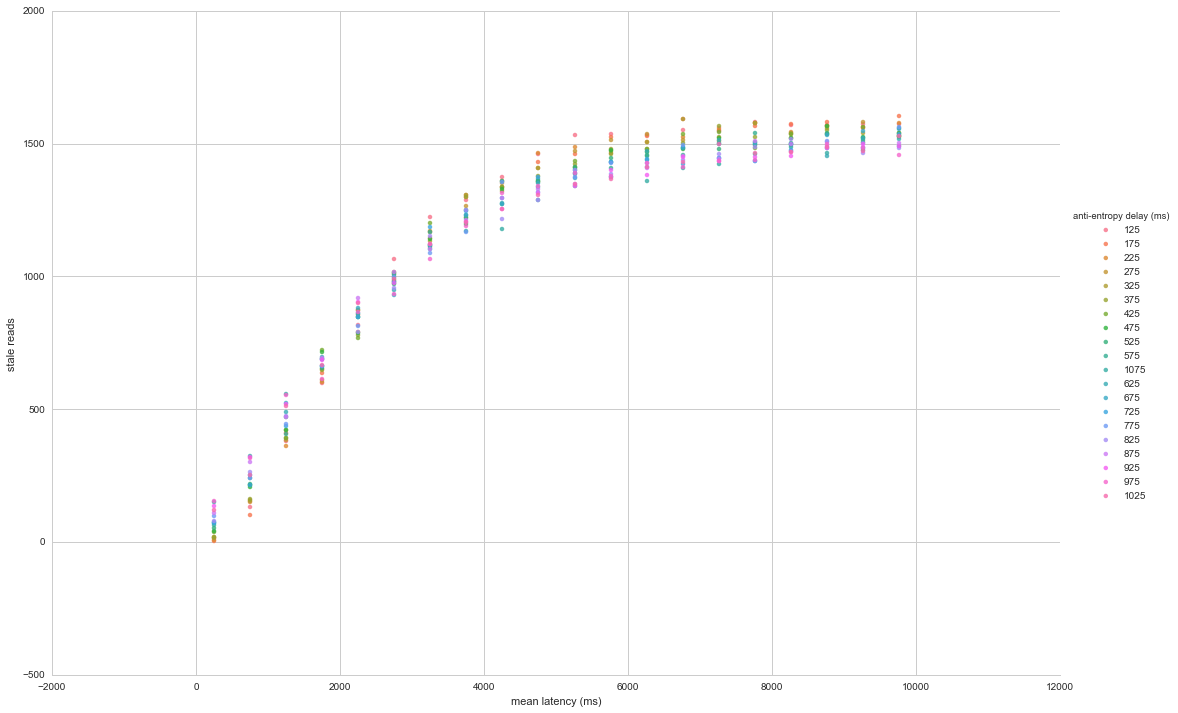
\includegraphics[width=0.5\textwidth]{figures/ae_stale_reads}
    \caption{Stale reads using eventual consistency with variable anti entropy delay.}
\end{figure}

\begin{figure}[h]
    \centering
    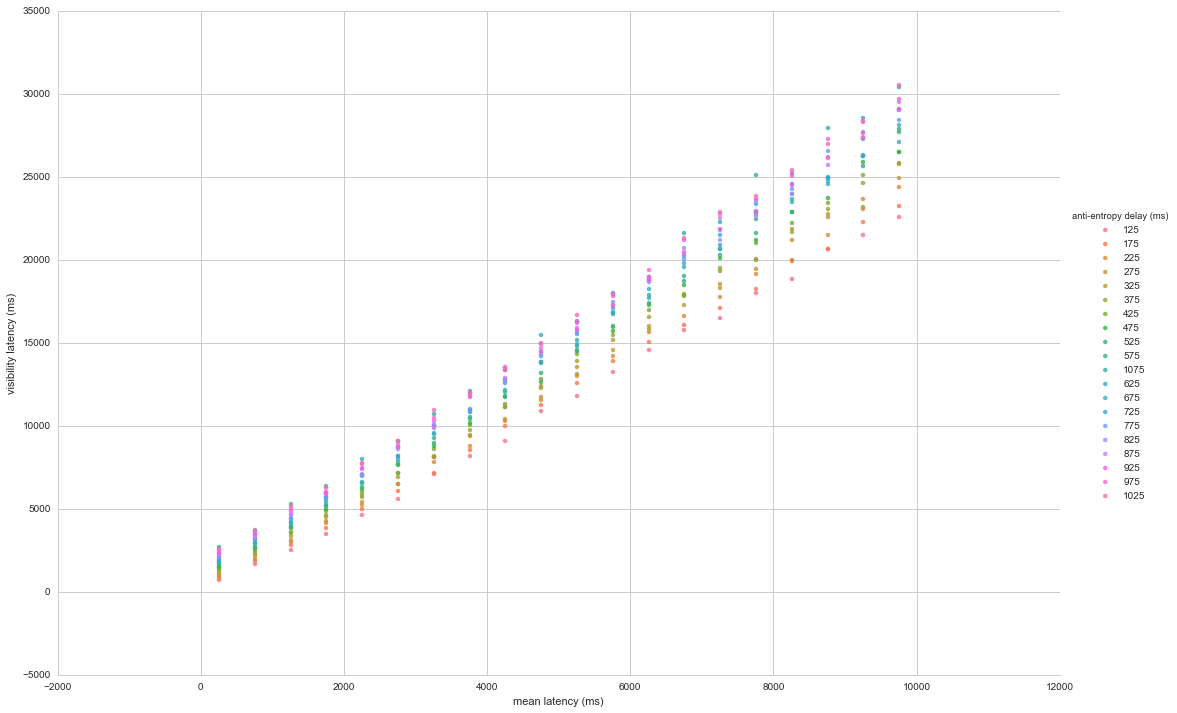
\includegraphics[width=0.5\textwidth]{figures/ae_viz_latency}
    \caption{Visibility latency using eventual consistency with variable anti entropy delay.}
\end{figure}

\begin{figure}[h]
    \centering
    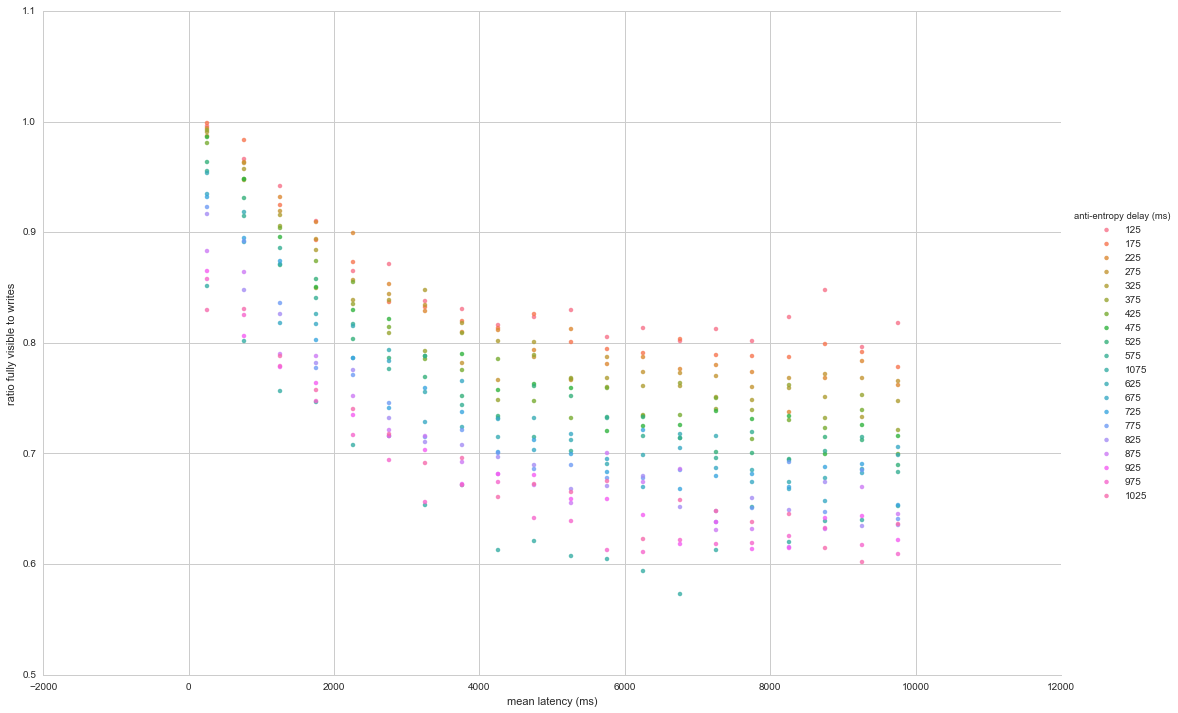
\includegraphics[width=0.5\textwidth]{figures/ae_viz_ratio}
    \caption{Ratio of fully visible writes to total writes using eventual consistency with variable anti entropy delay.}
\end{figure}

\begin{figure}[h]
    \centering
    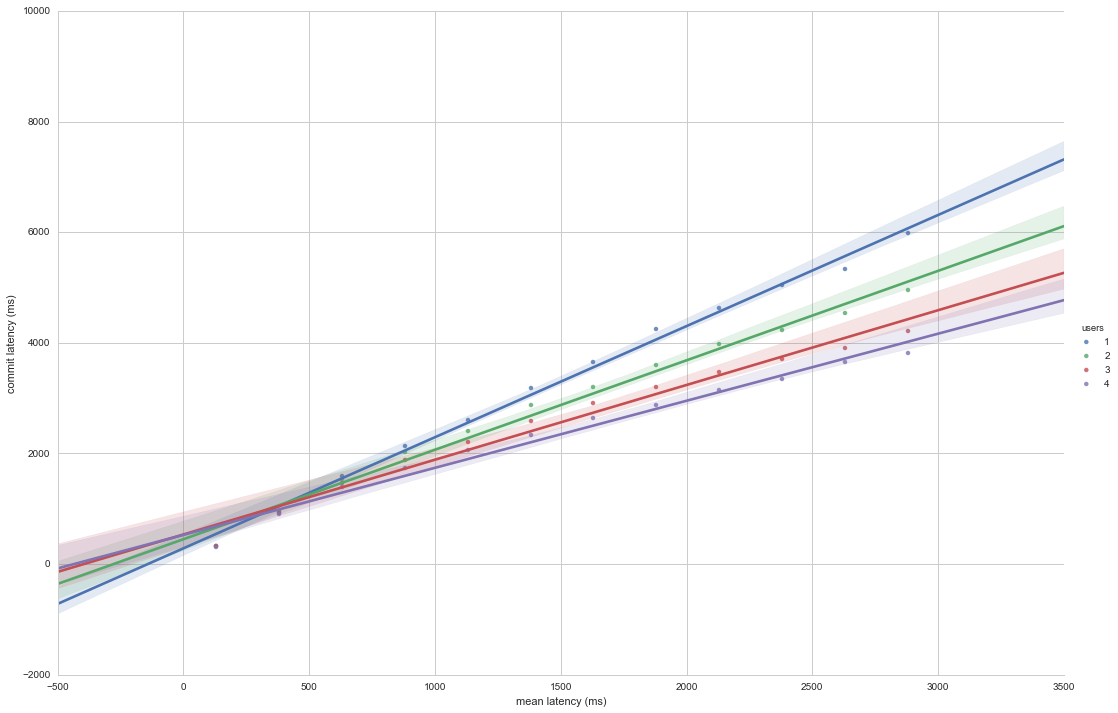
\includegraphics[width=0.5\textwidth]{figures/raft_commit_latency}
    \caption{Commit latency in Raft with increasing numbers of users.}
\end{figure}

\section{Conclusion}

\section*{Acknowledgments}

{\footnotesize \bibliographystyle{acm}
\bibliography{references}}

% uncomment to include end notes.
% \theendnotes

\end{document}
